\documentclass[12pt, letterpaper]{article}
% must use this pkg for displaying imgs
\usepackage{graphicx}
\graphicspath{ {../../imgs/} }
% pkg for links
\usepackage{hyperref}
% for codeblocks highlighting
\usepackage{listings}


\begin{document}


\newcommand{\paperauthor}{Akiel Aries}
\newcommand{\papersupervisor}{Prof. Sareh Assiri}
\newcommand{\paperuniversity}{Northern Arizona University}

\newcommand{\papertitle}{Analyzing Mirai}
\newcommand{\paperminortitle}{a *Nix-Focused Attack}
\newcommand{\papermajorheading}{Cybersecurity}
\newcommand{\paperminorheading}{CYB 410 - Software Security}

\newcommand{\HRule}{\rule{\linewidth}{0.5mm}} % Defines a new command for the horizontal lines, change thickness here

\center % Center everything on the page

%----------------------------------------------------------------------------------------
%	HEADING SECTIONS
%----------------------------------------------------------------------------------------

\textsc{\LARGE \paperuniversity}\\[1.0cm] % Name of your university/college
\textsc{\Large \papermajorheading}\\[0.2cm] % Major heading such as course name
\textsc{\large \paperminorheading}\\[0.75cm] % Minor heading such as course title

%----------------------------------------------------------------------------------------
%	TITLE SECTION
%----------------------------------------------------------------------------------------

\HRule \\[0.4cm]
{ \huge \bfseries \papertitle}\\[0.05cm] % Title of your document
{ \huge \paperminortitle}\\[0.025cm] % Title of your document
\HRule \\[3.5cm]

\begin{center}
	\makebox[0.8\textwidth]{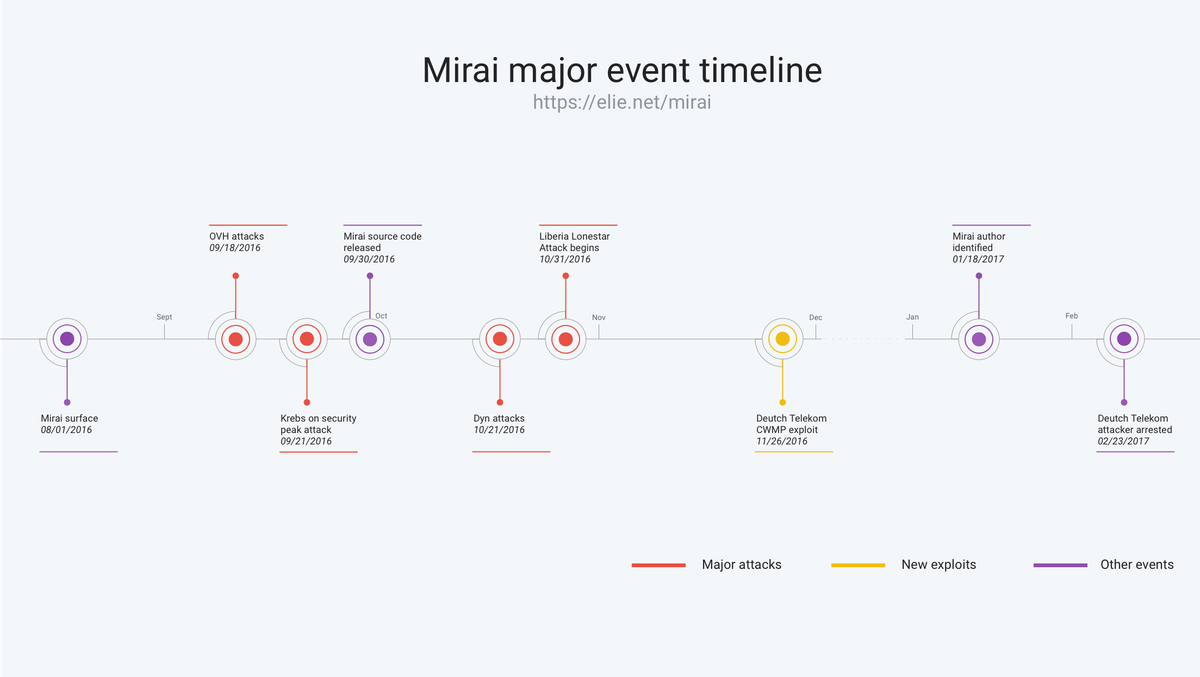
\includegraphics[width=0.8\textwidth]{mirai-major-events-timeline.png}}
\end{center}


\vfill % Fill the rest of the page with whitespace
%----------------------------------------------------------------------------------------
%	AUTHOR SECTION
%--------------------------------------------------------------------------------------

\begin{minipage}{0.4\textwidth}
	\begin{flushleft} \large
	\emph{Author:}\\
	\paperauthor
	\end{flushleft}
	\end{minipage}
	~
	\begin{minipage}{0.4\textwidth}
	\begin{flushright} \large
	\emph{Supervisor:} \\
	\papersupervisor
	\end{flushright}
\end{minipage}\\[1cm]

%----------------------------------------------------------------------------------------
%	DATE SECTION
%----------------------------------------------------------------------------------------
{\large \today}\\ % Date, change the \today to a set date if you want to be precise

\newpage

\begin{sloppypar}


% classification img
%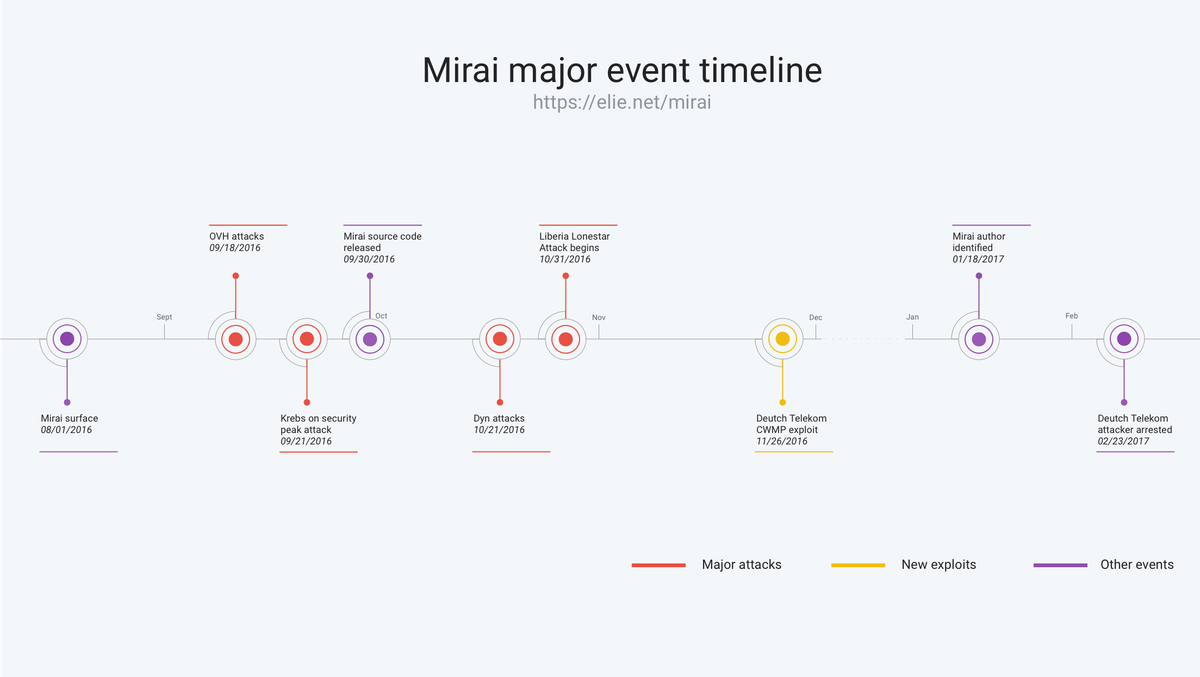
\includegraphics[scale=0.3]{mirai-major-events-timeline.png}

\section*{Introduction}
\begin{flushleft}
Mirai is a piece of malware targeting Internet of Things (IoT) devices first discovered 
in 2016 by a malware research group MalwareMustDie and gaining more popularity when 
cybersecurity journalist, Brian Krebs, had his website attacked. The goal being to 
control nodes part of a botnet running large-scale attacks. From previous research on 
attack history most victims include consumer grade devices such as local home routers 
and IP cameras, which are known to be insecure and attack-prone. The bot has been used 
in very large-scale DDoS (Distrubuted Denial of Service) atacks targeting many users 
machines and taking place accross the globe. Mirai's networking agent is written in C 
and its controller interface written in Go. It utilizes computer numerical control (CNC) 
which is a quite genius way to control the operation and functionality of a machine 
through injection of software. Since being discover and its source code leaked, Mirai 
went on to spawn many variations, much like pieces of malware, that exploited zero-day's 
in some pieces of software for effecient and malicious operation. 
\end{flushleft}

\section*{Code}
\begin{flushleft}
An interesting, and almost naive approach, is that Mirai makes use of dictionary attacks


Since Mirai is a DDOS bot, there are many spots in the code base of the bug that 
references some networking principles. The OSI (Open Systems Interconnection) model 
depicting the functions of a networking system. For now, let's take a look at how
Mirai makes use of layer 3, network. 
\begin{center}
{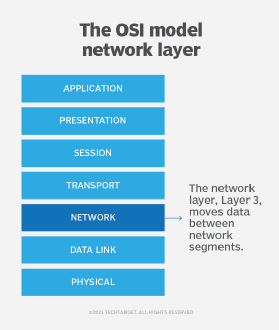
\includegraphics[width=0.8\textwidth]{osi-networking.png}}
\end{center}

Mirai makes use of launching GRE IP (Generic Routing Encapsulation) \& GRE ETH floods
in conjunction with SYN \& ACK floods.  


Interesting enough, within the code some addresses are hardcoded not to visit when
performing the IP scan for inital infection. Some of the 

\begin{verbatim}
static ipv4_t get_random_ip(void)
{
    uint32_t tmp;
    uint8_t o1, o2, o3, o4;

    do
    {
        tmp = rand_next();

        o1 = tmp & 0xff;
        o2 = (tmp >> 8) & 0xff;
        o3 = (tmp >> 16) & 0xff;
        o4 = (tmp >> 24) & 0xff;
    }
    while (o1 == 127 ||                             // 127.0.0.0/8      - Loopback
          (o1 == 0) ||                              // 0.0.0.0/8        - Invalid address space
          (o1 == 3) ||                              // 3.0.0.0/8        - General Electric Company
          (o1 == 15 || o1 == 16) ||                 // 15.0.0.0/7       - Hewlett-Packard Company
          (o1 == 56) ||                             // 56.0.0.0/8       - US Postal Service
          (o1 == 10) ||                             // 10.0.0.0/8       - Internal network
          (o1 == 192 && o2 == 168) ||               // 192.168.0.0/16   - Internal network
          (o1 == 172 && o2 >= 16 && o2 < 32) ||     // 172.16.0.0/14    - Internal network
          (o1 == 100 && o2 >= 64 && o2 < 127) ||    // 100.64.0.0/10    - IANA NAT reserved
          (o1 == 169 && o2 > 254) ||                // 169.254.0.0/16   - IANA NAT reserved
          (o1 == 198 && o2 >= 18 && o2 < 20) ||     // 198.18.0.0/15    - IANA Special use
          (o1 >= 224) ||                            // 224.*.*.*+       - Multicast
          (o1 == 6 || o1 == 7 || o1 == 11 || o1 == 21 || o1 == 22 || o1 == 26 || o1 == 28 
          || o1 == 29 || o1 == 30 || o1 == 33 || o1 == 55 || o1 == 214 || o1 == 215) 
          // Department of Defense
    );

    return INET_ADDR(o1,o2,o3,o4);
}

\end{verbatim}



This loop iterates through the ACK + SEQ numbers that are retrieved. SEQ is the value
sent by a TCP client that specifies the amount of data sent in the session. ACK is the 
value returned by the TCP server that indicates data has been recieved and is ready to
begin the next segment. 
\begin{verbatim}
// Retrieve all ACK/SEQ numbers
for (i = 0; i < targs_len; i++)
{
    int fd;
    struct sockaddr_in addr, recv_addr;
    socklen_t recv_addr_len;
    char pktbuf[256];
    time_t start_recv;

    stomp_setup_nums:

\end{verbatim}

Another important piece of the code is the hardcoding/bypassing taking place that 
implies more security risks. Mirai 


\begin{verbatim}

\end{verbatim}

This particular piece of the tcp attack file caught my attention and I found
that 0xffffffff is a Windows update error returning when the update fails to search
or install. 
\begin{verbatim}
if (source_ip == 0xffffffff)
	iph->saddr = rand_next();
\end{verbatim}

\end{flushleft}


\section*{Scale}
\begin{flushleft}
It was reported that the Mirai virus was located in 160+ countries.
Geolocations of devices infected by Mirai

\begin{center}
\begin{tabular}{c c}
Vietnam	& 12.8 \%\\
Brazil & 11.8 \%\\
United States & 10.9 \%\\
China & 8.8 \%\\
Mexico & 8.4 \%\\
South Korea	& 6.2 \%\\
Taiwan & 4.9 \%\\
Russia & 4.0 \%\\
Romania	& 2.3 \%\\
Colombia	 & 1.5 \%\\
\end{tabular}
\end{center}

\end{flushleft}


\section*{Running the Bug}
\begin{flushleft}

Requirements: \\
\begin{itemize}
\item 2 servers: 1 for CNC + mysql, 1 for scan receiver, and 1+ for loading
\end{itemize}

Setup
\begin{itemize}
\item 2 VPS and 4 servers
\item 1 VPS with extremely bulletproof host for database server
\item 1 VPS, rootkitted, for scanReceiver and distributor
\item 1 server for CNC (used like 2% CPU with 400k bots)
\item 3x 10gbps NForce servers for loading (distributor distributes to 3 servers equally)
\end{itemize}



\end{flushleft}



\section*{Static Analysis/Debugging}
\begin{flushleft}


\end{flushleft}


\section*{Final Notes}
\begin{flushleft}



\end{flushleft}


\section*{Sources}
\begin{flushleft}
https://www.imperva.com/blog/malware-analysis-mirai-ddos-botnet/
https://blog.malwaremustdie.org/2016/08/mmd-0056-2016-linuxmirai-just.html

\end{flushleft}



\end{sloppypar}
\end{document}
